\subsubsection{Augmented Reality}
Augmented Reality er en teknologi der kan sætte virtuelle objekter ind i en virkelig kontekst. Derudover har man mulighed for at interagere med objektet i real tid.
Augmented Reality kan direkte oversættes til "Fordrejet virkelighed". Augmented reality bruges i blandt andet jægerfly \cite{hud} hvor en "HUD" (Head-Up Display) bruges til at fortælle piloten informationer om højde, hastighed (se figur) men kan også bruges til at vise en landingsbane hvis det f.eks. er tåget og man ikke kan se landingsbanen. 
Vi ser også Augmented Reality i hverdagen hvor f.eks. redigerede billeder på Instagram er en form for augmented reality. I takt med at billig computerkraft er blevet hvermands-eje er Augmented Reality også på vej ind i spil-verdenen hvor en kedelig skov eller mark kan blive til en skydebane hvor man kan spille mod sine venner.

\begin{figure}[H]
    \centering
    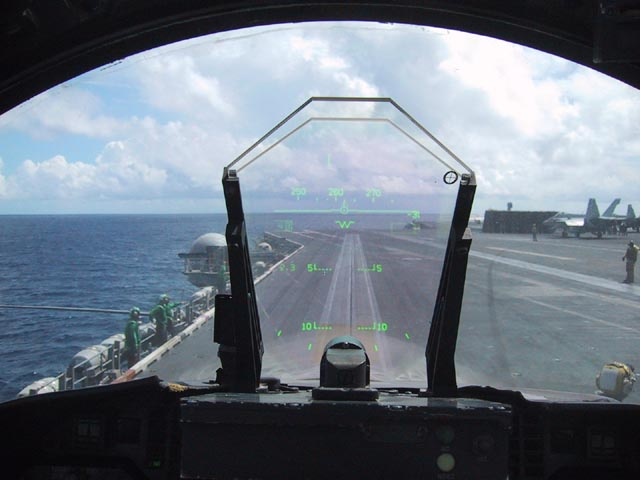
\includegraphics[width=10cm]{hud.jpg}
    \caption{Heads-Up Display fra et "F/A-18 Hornet" jægerfly}
    \label{fig:hud}
\end{figure} 
